O segundo teste (Figura \ref{fig:teste1}) mostra o impacto na mudan�a do n�mero de \emph{octaves}, considerando o n�mero de terrenos vizinhos fixo em 2. As quedas abruptas de rendimento significam momentos em que a gera��o dos novos terrenos est� acontecendo. Quanto maior o n�mero de \emph{octaves}, maior o n�mero de v�rtices da malha do terreno; explicando assim o FPS menor.

\begin{figure}[H]
	\center{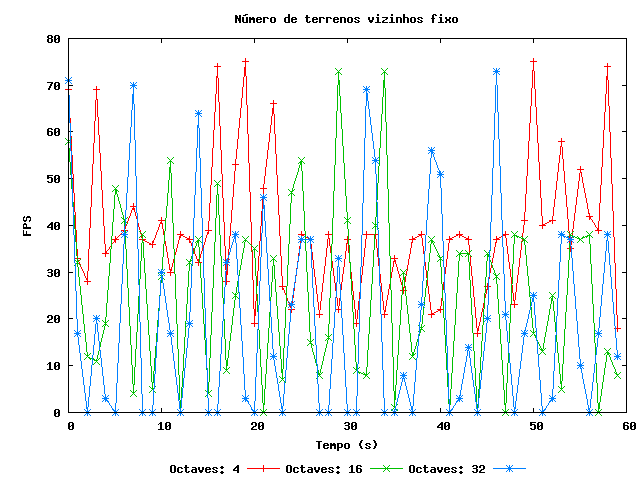
\includegraphics[width=0.5\linewidth]{img/graficos/teste1/teste1.png}}
	\caption{\label{fig:teste1} Teste variando o n�mero de \emph{octaves}, e o n�mero de terrenos vizinhos fixo em 2.}
\end{figure}